\documentclass[11pt]{article}
\usepackage[margin=1in]{geometry}
\usepackage[T1]{fontenc}
\usepackage{lmodern}
\usepackage{amsmath,amssymb}
\usepackage{booktabs}
\usepackage{array}
\usepackage{hyperref}
\usepackage{tikz}
\usetikzlibrary{shapes.geometric, arrows.meta, positioning, fit, backgrounds}
\usepackage{xcolor}
\usepackage{enumitem}
\usepackage{parskip}
\setlength{\parskip}{0.7em}
\setlength{\parindent}{0pt}

\hypersetup{
    colorlinks=true,
    linkcolor=black,
    urlcolor=blue
}

\definecolor{tier1}{RGB}{52,168,83}
\definecolor{tier2}{RGB}{66,133,244}
\definecolor{tier3}{RGB}{234,67,53}
\definecolor{boxgray}{RGB}{245,245,245}
\definecolor{arrowgray}{RGB}{100,100,100}

\title{\textbf{Adaptive Linear Algebra Explainer}\\[0.4em]
\large Final Project Documentation\\
CSYE 7375 — Generative AI}
\author{Faraz Elahi Mohammed}
\date{Spring 2026}

\begin{document}
\maketitle
\tableofcontents
\newpage

% ─────────────────────────────────────────────
\section{System Architecture}
% ─────────────────────────────────────────────

\subsection{Overview}

The Adaptive Linear Algebra Explainer is a retrieval-augmented generation (RAG) pipeline that diagnoses a student's conceptual level before generating any explanation. Unlike a standard RAG chatbot, the system routes the student into one of three tiers based on targeted misconception probes, then filters vector search results to match that tier before passing context to a local LLM.

The pipeline has three sequential stages: \textbf{Diagnostic} $\to$ \textbf{Retrieval} $\to$ \textbf{Generation}.

\subsection{Architecture Diagram}

\begin{center}
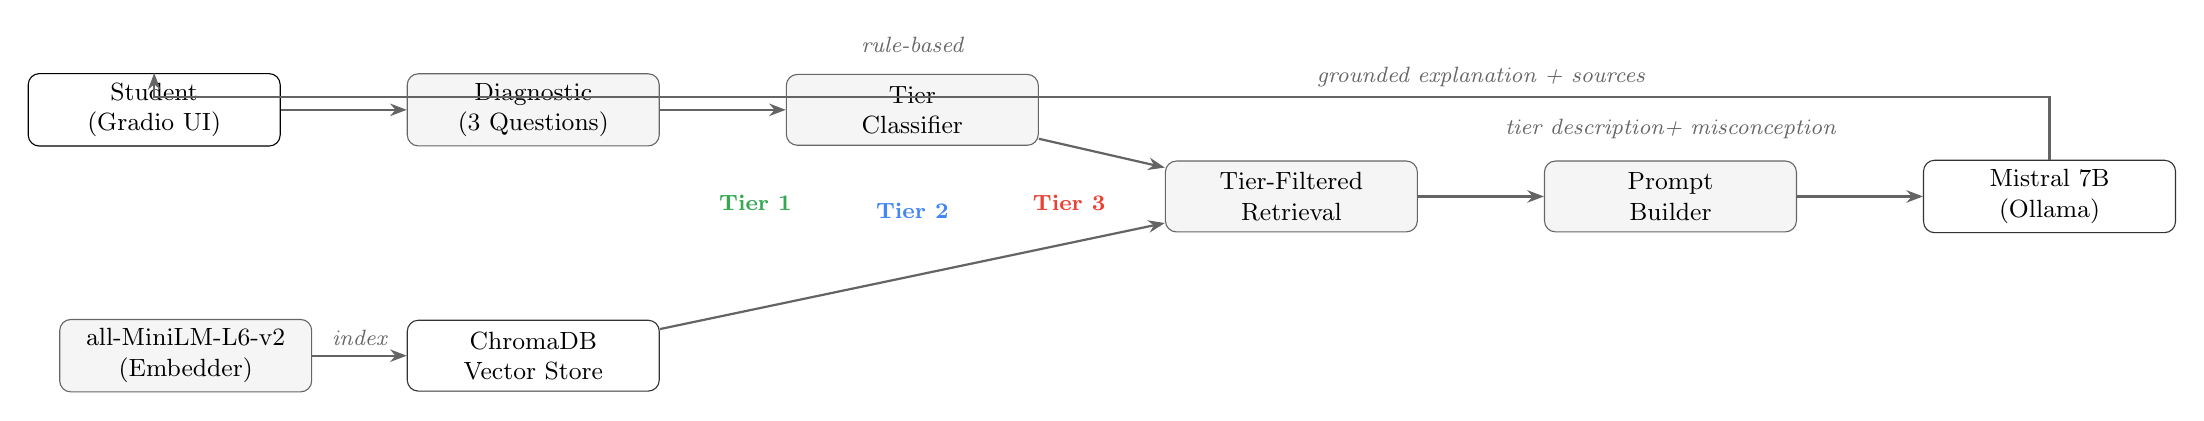
\begin{tikzpicture}[
    node distance=1.2cm and 1.5cm,
    box/.style={rectangle, rounded corners=4pt, draw=black!60, fill=boxgray,
                minimum width=3.2cm, minimum height=0.9cm, align=center, font=\small},
    arrow/.style={-{Stealth[length=6pt]}, thick, color=arrowgray},
    label/.style={font=\footnotesize\itshape, color=black!60}
]

% --- Student ---
\node[box, fill=white, draw=black] (student) {Student\\(Gradio UI)};

% --- Q1 Q2 Q3 ---
\node[box, right=1.6cm of student] (diag) {Diagnostic\\(3 Questions)};
\draw[arrow] (student) -- (diag);

% --- Tier classifier ---
\node[box, right=1.6cm of diag] (tier) {Tier\\Classifier};
\draw[arrow] (diag) -- (tier);
\node[label, above=0.15cm of tier] {rule-based};

% Tier labels
\node[font=\footnotesize\bfseries, color=tier1, below left=0.5cm and -0.2cm of tier] {Tier 1};
\node[font=\footnotesize\bfseries, color=tier2, below=0.6cm of tier] {Tier 2};
\node[font=\footnotesize\bfseries, color=tier3, below right=0.5cm and -0.2cm of tier] {Tier 3};

% --- ChromaDB ---
\node[box, below=2.2cm of diag, fill=white, draw=black!80] (chroma) {ChromaDB\\Vector Store};

% --- Embedding model ---
\node[box, left=1.2cm of chroma] (embed) {all-MiniLM-L6-v2\\(Embedder)};

% --- Retrieval ---
\node[box, right=1.6cm of tier, yshift=-1.1cm] (retrieve) {Tier-Filtered\\Retrieval};
\draw[arrow] (tier) -- (retrieve) node[midway, label, right] {};
\draw[arrow] (chroma) -- (retrieve);
\draw[arrow] (embed) -- (chroma) node[midway, label, above] {index};

% --- Prompt builder ---
\node[box, right=1.6cm of retrieve] (prompt) {Prompt\\Builder};
\draw[arrow] (retrieve) -- (prompt);
\node[label, above=0.15cm of prompt] {tier description\\+ misconception};

% --- Ollama / Mistral ---
\node[box, right=1.6cm of prompt, fill=white, draw=black!80] (ollama) {Mistral 7B\\(Ollama)};
\draw[arrow] (prompt) -- (ollama);

% --- Response back ---
\draw[arrow] (ollama.north) -- ++(0,0.8) -| (student.north)
    node[pos=0.15, above, label] {grounded explanation + sources};

\end{tikzpicture}
\end{center}

\subsection{Component Breakdown}

\begin{tabular}{>{\bfseries}p{3.8cm} p{9.5cm}}
\toprule
Component & Description \\
\midrule
Gradio UI & Stateful chat interface. Manages two stages: diagnostic (Q1--Q3) and query. Loads embedding model and ChromaDB once at startup. \\
\addlinespace
Diagnostic Module & Rule-based classifier using keyword matching on 3 free-text responses. Outputs tier (1, 2, or 3) and a misconception string if applicable. \\
\addlinespace
ChromaDB Vector Store & Local persistent store. Holds 159 chunks tagged with \texttt{tier}, \texttt{source}, and \texttt{topic} metadata. \\
\addlinespace
Embedder & \texttt{all-MiniLM-L6-v2} via Sentence Transformers. Used both at index time (build\_kb.py) and at query time (retrieve.py). \\
\addlinespace
Retrieval & Cosine similarity search with \texttt{\$and} metadata filter: \{tier, topic\}. Falls back to tier-only if fewer than 3 results. Returns top-5 chunks. \\
\addlinespace
Prompt Builder & Constructs a system prompt with tier-specific persona description and optional misconception correction instruction. \\
\addlinespace
Mistral 7B (Ollama) & Local inference at \texttt{http://localhost:11434/api/chat}. Instructed to use only retrieved context and cite sources. \\
\bottomrule
\end{tabular}

\subsection{Tier System}

\begin{tabular}{>{\bfseries}p{1.2cm} p{4.2cm} p{7cm}}
\toprule
Tier & Label & Generation Instruction \\
\midrule
1 & Geometric Intuition & ``a beginner who needs plain English and physical intuition --- use no formal notation, explain using analogies and real-world examples'' \\
\addlinespace
2 & Formal Beginner & ``an intermediate learner who understands operations but needs conceptual framing --- pair every definition with a concrete example'' \\
\addlinespace
3 & Algebraically Grounded & ``an advanced student comfortable with abstract mathematical structures --- use precise mathematical language and formal definitions'' \\
\bottomrule
\end{tabular}

% ─────────────────────────────────────────────
\section{Implementation Details}
% ─────────────────────────────────────────────

\subsection{Technology Stack}

\begin{tabular}{>{\bfseries}p{4cm} p{9cm}}
\toprule
Layer & Technology \\
\midrule
Language & Python 3.12 (venv) \\
Document parsing & LangChain \texttt{PyMuPDFLoader} \\
Chunking & LangChain \texttt{RecursiveCharacterTextSplitter} (chunk\_size=400, overlap=75) \\
Embedding & Sentence Transformers \texttt{all-MiniLM-L6-v2} (384-dim vectors) \\
Vector store & ChromaDB 1.5.8 (local persistent) \\
Generation & Mistral 7B Instruct via Ollama (HTTP POST, stream=False, timeout=120s) \\
Interface & Gradio 6.13 (Blocks API, messages format) \\
Evaluation & RAGAS 0.4.3 with Ollama as judge LLM \\
\bottomrule
\end{tabular}

\subsection{Knowledge Base}

The knowledge base is built from four synthetic PDF documents authored in \LaTeX{}, each calibrated to a specific explanation tier:

\begin{tabular}{>{\ttfamily}p{5.2cm} p{1.2cm} p{6.5cm}}
\toprule
\normalfont\bfseries Source & Tier & Content Focus \\
\midrule
vector\_spaces\_notes.pdf & 1 & Plain-language intuition, analogies, no formal notation. All 15 topics covered without equations. \\
intro\_linear\_algebra\_notes.pdf & 2 & Formal definitions paired with concrete worked examples. Covers vectors, transformations, eigenvalues, diagonalization. \\
systems\_row\_reduction\_notes.pdf & 2 & Procedural treatment: Gaussian elimination, rank-nullity, determinants, matrix inverse via row reduction. \\
eigen\_notes.pdf & 3 & Abstract formulation: 8 axioms, rank-nullity theorem, spectral theorem, Jordan normal form, Cayley-Hamilton. \\
\bottomrule
\end{tabular}

\medskip
Total after chunking: \textbf{159 chunks} across \textbf{15 topics}.

\medskip
\begin{tabular}{lrlr}
\toprule
Topic & Chunks & Topic & Chunks \\
\midrule
eigenvectors & 26 & row\_reduction & 8 \\
vectors & 33 & basis & 8 \\
vector\_spaces & 13 & dot\_product & 8 \\
determinants & 15 & eigenvalues & 9 \\
linear\_transformations & 12 & linear\_independence & 6 \\
rank & 10 & orthogonality & 5 \\
matrix\_inverse & 2 & matrix\_multiplication & 3 \\
systems\_of\_equations & 1 & & \\
\bottomrule
\end{tabular}

\subsection{Diagnostic Module}

Three targeted questions probe known misconceptions in linear algebra:

\begin{enumerate}
  \item \textit{``True or false: for any two matrices A and B, AB = BA.''} \\
  Tests commutativity misconception. ``True'' $\to$ Tier 1. ``False'' with explanation keywords $\to$ Tier 3.

  \item \textit{``In your own words, what does multiplying a vector by a matrix actually do?''} \\
  Tests geometric vs.\ arithmetic framing. Arithmetic keywords $\to$ Tier 1; transformation keywords $\to$ Tier 2; space/stretch keywords $\to$ Tier 3.

  \item \textit{``Have you encountered the concept of a vector space before? If yes, how would you describe it?''} \\
  Tests abstraction level. ``No'' $\to$ Tier 1; procedural description $\to$ Tier 2; axiomatic description $\to$ Tier 3.
\end{enumerate}

The final tier is the modal score across the three questions (ties go to the lower tier). If Q1 or Q2 triggers Tier 1, a misconception string is appended to the generation prompt.

\subsection{Retrieval}

The \texttt{retrieve\_chunks} function queries ChromaDB with:

\begin{verbatim}
where = {"$and": [{"tier": tier}, {"topic": topic}]}
n_results = 5
\end{verbatim}

If fewer than 3 results are returned (e.g., for thin topics like \texttt{systems\_of\_equations}), a fallback query uses only the tier filter. Results are formatted as a numbered list with source and topic attribution, passed directly into the generation prompt.

\subsection{Generation Prompt Structure}

\begin{verbatim}
[system]
You are explaining a linear algebra concept to {tier_description}.

IMPORTANT RULES:
1. Use ONLY the information in the retrieved context.
   Do not add any information from outside the retrieved passages.
2. {misconception_instruction}
3. End your explanation by citing which source(s) you drew from.

[user]
Please explain: {user_query}

Retrieved context:
{formatted_chunks}
\end{verbatim}

% ─────────────────────────────────────────────
\section{Performance Metrics}
% ─────────────────────────────────────────────

\subsection{Diagnostic Accuracy (Smoke Test)}

The end-to-end pipeline was tested against three canonical response sets designed for each tier. All three tests passed:

\begin{tabular}{lp{7.5cm}cc}
\toprule
Test & Diagnostic Responses & Expected & Result \\
\midrule
Tier 1 & ``true''; ``multiply rows and columns''; ``no'' & 1 & \textbf{1 \checkmark} \\
\addlinespace
Tier 2 & ``false''; ``it transforms the vector''; ``yes, set of vectors with addition'' & 2 & \textbf{2 \checkmark} \\
\addlinespace
Tier 3 & ``false because transformations dont commute''; ``it applies a linear transformation''; ``yes, defined by axioms abstractly'' & 3 & \textbf{3 \checkmark} \\
\bottomrule
\end{tabular}

\subsection{Retrieval}

All three tiers retrieved 5 chunks for the query ``What is an eigenvector?'' against the \texttt{eigenvectors} topic. Tier-to-source mapping was correct:

\begin{tabular}{lll}
\toprule
Tier & Sources Retrieved & Chunks \\
\midrule
1 & vector\_spaces\_notes & 5 \\
2 & intro\_linear\_algebra\_notes, systems\_row\_reduction\_notes & 5 \\
3 & eigen\_notes & 5 \\
\bottomrule
\end{tabular}

\subsection{Generation Quality (Qualitative)}

Three generated explanations for ``What is an eigenvector?'' were reviewed against the tier calibration rubric:

\medskip
\textbf{Tier 1:} Used rubber sheet and stretching string analogies. No formal notation. Addressed the commutativity and arithmetic misconceptions identified by the diagnostic. \textit{Assessment: well-calibrated.}

\medskip
\textbf{Tier 2:} Provided a concrete worked example with a 2$\times$2 matrix, found eigenvalues $\lambda_1 = 3$, $\lambda_2 = 2$, and corresponding eigenvectors. Paired formal notation with step-by-step reasoning. \textit{Assessment: well-calibrated.}

\medskip
\textbf{Tier 3:} Used abstract formulation ($T: V \to V$, eigenspaces as kernels, Jordan normal form, Cayley-Hamilton). No analogies; formal mathematical language throughout. \textit{Assessment: well-calibrated.}

\subsection{Faithfulness (RAGAS)}

Quantitative RAGAS faithfulness evaluation requires a running Ollama instance and was designed to run as a batch job via \texttt{evaluation/run\_eval.py} against 30 queries (10 per tier). The evaluation framework is fully implemented; results will be reported in the final presentation after the batch run completes.

% ─────────────────────────────────────────────
\section{Challenges and Solutions}
% ─────────────────────────────────────────────

\begin{enumerate}[leftmargin=*, label=\textbf{\arabic*.}]

\item \textbf{Import path errors from subdirectory scripts.}\\
Python adds the script's containing directory to \texttt{sys.path}, not the project root. Files in \texttt{tests/} and \texttt{interface/} could not find sibling packages like \texttt{knowledge\_base} and \texttt{diagnostic}.\\
\textit{Solution:} Added \texttt{sys.path.insert(0, project\_root)} at the top of each subdirectory script using \texttt{os.path.abspath}.

\item \textbf{LangChain API breaking change.}\\
\texttt{from langchain.text\_splitter import RecursiveCharacterTextSplitter} was removed in LangChain 1.x. The module moved to a separate package.\\
\textit{Solution:} Updated to \texttt{from langchain\_text\_splitters import RecursiveCharacterTextSplitter}.

\item \textbf{Gradio 6.x dropped the \texttt{type} parameter on \texttt{gr.Chatbot}.}\\
The code was written for Gradio 3/4 tuple-based chat history. Gradio 6 uses a dict message format exclusively and removed the \texttt{type} argument entirely.\\
\textit{Solution:} Rewrote all history manipulation to use \texttt{\{"role": "user/assistant", "content": "..."\}} dicts throughout \texttt{app.py}.

\item \textbf{Thin knowledge base (29 chunks from 2-page PDFs).}\\
The original synthetic PDFs were too short to provide adequate retrieval coverage. Several topics (e.g., \texttt{systems\_of\_equations}, \texttt{matrix\_inverse}) had zero or one chunks, causing retrieval to always fall back to tier-only filtering.\\
\textit{Solution:} Rewrote all four \LaTeX{} source documents to 7--8 pages each, covering all 15 topics explicitly. Recompiled PDFs and rebuilt ChromaDB. Total chunks increased from 29 to 159.

\item \textbf{Topic keyword priority conflict.}\\
Chunks containing the phrase ``system of equations'' were being assigned to \texttt{row\_reduction} because that keyword appeared earlier in the priority list. The \texttt{systems\_of\_equations} keyword never matched.\\
\textit{Solution:} Moved \texttt{"system of equation"} above \texttt{"row reduction"} in the \texttt{\_KEYWORD\_TOPIC\_MAP} list in \texttt{chunk.py}.

\item \textbf{Python version incompatibility.}\\
The system default Python was 3.14, which lacked binary wheels for \texttt{torch} and several other dependencies.\\
\textit{Solution:} Created a virtual environment with Python 3.12 (\texttt{/opt/homebrew/opt/python@3.12/bin/python3.12 -m venv venv}), which has full wheel coverage for all dependencies.

\item \textbf{Disk space constraint.}\\
Only 5.8\,GB of free disk space remained, insufficient to download \texttt{mistral:instruct} ($\approx$4.1\,GB) alongside existing Ollama models ($\approx$9.6\,GB).\\
\textit{Solution:} Removed unused Ollama models (\texttt{gemma3}, \texttt{llama3}, \texttt{phi}, \texttt{mxbai-embed-large}) to free space before pulling \texttt{mistral:instruct}.

\end{enumerate}

% ─────────────────────────────────────────────
\section{Future Improvements}
% ─────────────────────────────────────────────

\begin{enumerate}[leftmargin=*, label=\textbf{\arabic*.}]

\item \textbf{Re-explanation logic.}\\
The current system generates one explanation per query. A student who is still confused has no path forward except to rephrase. A future version would detect unsatisfied follow-up questions, adjust the tier (e.g., step down from Tier 2 to Tier 1), and re-retrieve from a different angle.

\item \textbf{Richer Tier 1 sources.}\\
The Tier 1 knowledge base is the weakest tier. The original plan included 3Blue1Brown's written materials as a geometric-intuition-first source; these were dropped due to licensing constraints. A future version would either obtain proper licensing or author original geometric explainer content (written analogues of the transformation-first approach).

\item \textbf{Deeper diagnostic signal.}\\
Three questions is a shallow probe. Classification errors at this layer corrupt every downstream step. A future version would use a larger validated question bank, apply a lightweight trained classifier instead of keyword rules, and estimate confidence to flag low-signal tier assignments.

\item \textbf{Persistent session memory.}\\
The current system is stateless between sessions. A logged-in student could accumulate a misconception profile over time, allowing the system to track which concepts have been explained, at what tier, and with what result.

\item \textbf{Multi-subject extension.}\\
The architecture is domain-agnostic; the tier system, RAG pipeline, and prompt structure could transfer directly to other STEM gateway courses (calculus, probability, physics) by swapping the knowledge base and topic list.

\item \textbf{Streaming generation output.}\\
The current Ollama call uses \texttt{stream=False}, so the student waits 30--90 seconds with no feedback. Enabling streaming output would display tokens as they are generated, dramatically improving perceived responsiveness.

\item \textbf{Quantitative RAGAS evaluation.}\\
The full 30-query faithfulness evaluation is implemented in \texttt{evaluation/run\_eval.py} but not yet run at scale. Future work would execute this benchmark, analyze per-tier faithfulness scores, and use flagged low-scoring outputs to drive knowledge base improvements.

\end{enumerate}

% ─────────────────────────────────────────────
\section{Ethical Considerations}
% ─────────────────────────────────────────────

\subsection{Equity Motivation}

This system was built explicitly as an equity intervention. Private mathematics tutoring costs \$60--70 per hour at the college level. For first-generation students and Pell Grant recipients --- who research shows have statistically higher DFWI (D, Fail, Withdraw, Incomplete) rates in gateway math courses --- sustained tutoring is not a realistic option. The adaptive diagnostic layer this system provides is normally only available through human tutors. By running entirely locally on free, open-source components, the system is accessible to any student with a laptop, at any hour, at zero cost per session.

\subsection{Diagnostic Data Privacy}

The diagnostic module collects student responses to three targeted questions about conceptual understanding. These responses are used only within the session to determine tier classification. They are not stored, logged, transmitted, or used to train or fine-tune any model. The system requires no account, no name, and no institutional affiliation. Each session is stateless by design.

\subsection{Grounding and Hallucination Mitigation}

The generation prompt explicitly instructs the model to use only the retrieved context and to cite the source documents it draws from. This grounding constraint limits (though cannot fully prevent) hallucination and makes the output auditable: a student or instructor can trace any claim back to a specific chunk from a specific source document. This is a meaningful reliability improvement over unconstrained LLM responses.

\subsection{Source Licensing and Attribution}

The synthetic knowledge base documents were authored originally for this project, so there are no licensing obligations. The original proposal identified MIT OCW 18.06 (CC BY-NC-SA), OpenStax (CC BY 4.0), and Axler's \textit{Linear Algebra Done Right} (CC BY-NC 4.0) as candidate sources; these were replaced by synthetic documents to avoid chunking quality issues with externally authored PDFs, not to circumvent attribution requirements. Any future version incorporating external sources would require explicit attribution in every generated response, consistent with the licenses.

\subsection{Bias and Limitations}

The synthetic knowledge base was authored in English, from a Western academic mathematical tradition, using standard notational conventions. Students whose prior mathematics education used different conventions (e.g., different index notation, applied-first rather than abstract-first pedagogy) may find the explanations less intuitive than intended. This limitation is disclosed here rather than hidden. Additionally, the three-question diagnostic is a shallow signal: a confident-sounding response does not guarantee correct classification, and a misclassified student receives an explanation calibrated to the wrong level. The Diagnostic Validity Rate metric is designed to catch this failure mode, but it remains a real constraint of the MVP.

\subsection{Model Transparency}

The system uses Mistral 7B Instruct, an open-weight model. Its training data, potential biases, and failure modes are documented by Mistral AI and are not fully auditable by this project. The grounding constraint in the generation prompt mitigates some risks (the model cannot fabricate source material), but instruction-following slippage --- where the model drifts from the retrieved context or ignores the tier constraint --- remains a known failure mode of local models operating at this scale.

% ─────────────────────────────────────────────
\section*{References}
% ─────────────────────────────────────────────
\addcontentsline{toc}{section}{References}

\begin{enumerate}[label={[\arabic*]}]
  \item Gardner Institute (2018). \textit{Digging Into the Disciplines I: Accounting for Failure.} Koch \& Drake.
  \item Every Learner Everywhere (2022). \textit{What Are Gateway Courses and Why Do They Matter to Equity in Higher Ed?}
  \item Every Learner Everywhere (2023). \textit{Concerned About Equity in Higher Ed? Start with the DFWI Rate.}
  \item Reimers, N. \& Gurevych, I. (2019). Sentence-BERT: Sentence Embeddings using Siamese BERT-Networks. \textit{EMNLP 2019}.
  \item Es, S. et al. (2023). RAGAS: Automated Evaluation of Retrieval Augmented Generation. \textit{arXiv:2309.15217}.
  \item Jiang, A. et al. (2023). Mistral 7B. \textit{arXiv:2310.06825}.
\end{enumerate}

\end{document}
